% Options for packages loaded elsewhere
\PassOptionsToPackage{unicode}{hyperref}
\PassOptionsToPackage{hyphens}{url}
%
\documentclass[
  ignorenonframetext,
]{beamer}
\usepackage{pgfpages}
\setbeamertemplate{caption}[numbered]
\setbeamertemplate{caption label separator}{: }
\setbeamercolor{caption name}{fg=normal text.fg}
\beamertemplatenavigationsymbolsempty
% Prevent slide breaks in the middle of a paragraph
\widowpenalties 1 10000
\raggedbottom
\setbeamertemplate{part page}{
  \centering
  \begin{beamercolorbox}[sep=16pt,center]{part title}
    \usebeamerfont{part title}\insertpart\par
  \end{beamercolorbox}
}
\setbeamertemplate{section page}{
  \centering
  \begin{beamercolorbox}[sep=12pt,center]{part title}
    \usebeamerfont{section title}\insertsection\par
  \end{beamercolorbox}
}
\setbeamertemplate{subsection page}{
  \centering
  \begin{beamercolorbox}[sep=8pt,center]{part title}
    \usebeamerfont{subsection title}\insertsubsection\par
  \end{beamercolorbox}
}
\AtBeginPart{
  \frame{\partpage}
}
\AtBeginSection{
  \ifbibliography
  \else
    \frame{\sectionpage}
  \fi
}
\AtBeginSubsection{
  \frame{\subsectionpage}
}

\usepackage{amsmath,amssymb}
\usepackage{lmodern}
\usepackage{iftex}
\ifPDFTeX
  \usepackage[T1]{fontenc}
  \usepackage[utf8]{inputenc}
  \usepackage{textcomp} % provide euro and other symbols
\else % if luatex or xetex
  \usepackage{unicode-math}
  \defaultfontfeatures{Scale=MatchLowercase}
  \defaultfontfeatures[\rmfamily]{Ligatures=TeX,Scale=1}
\fi
% Use upquote if available, for straight quotes in verbatim environments
\IfFileExists{upquote.sty}{\usepackage{upquote}}{}
\IfFileExists{microtype.sty}{% use microtype if available
  \usepackage[]{microtype}
  \UseMicrotypeSet[protrusion]{basicmath} % disable protrusion for tt fonts
}{}
\makeatletter
\@ifundefined{KOMAClassName}{% if non-KOMA class
  \IfFileExists{parskip.sty}{%
    \usepackage{parskip}
  }{% else
    \setlength{\parindent}{0pt}
    \setlength{\parskip}{6pt plus 2pt minus 1pt}}
}{% if KOMA class
  \KOMAoptions{parskip=half}}
\makeatother
\usepackage{xcolor}
\newif\ifbibliography
\setlength{\emergencystretch}{3em} % prevent overfull lines
\setcounter{secnumdepth}{-\maxdimen} % remove section numbering


\providecommand{\tightlist}{%
  \setlength{\itemsep}{0pt}\setlength{\parskip}{0pt}}\usepackage{longtable,booktabs,array}
\usepackage{calc} % for calculating minipage widths
\usepackage{caption}
% Make caption package work with longtable
\makeatletter
\def\fnum@table{\tablename~\thetable}
\makeatother
\usepackage{graphicx}
\makeatletter
\def\maxwidth{\ifdim\Gin@nat@width>\linewidth\linewidth\else\Gin@nat@width\fi}
\def\maxheight{\ifdim\Gin@nat@height>\textheight\textheight\else\Gin@nat@height\fi}
\makeatother
% Scale images if necessary, so that they will not overflow the page
% margins by default, and it is still possible to overwrite the defaults
% using explicit options in \includegraphics[width, height, ...]{}
\setkeys{Gin}{width=\maxwidth,height=\maxheight,keepaspectratio}
% Set default figure placement to htbp
\makeatletter
\def\fps@figure{htbp}
\makeatother

\makeatletter
\makeatother
\makeatletter
\makeatother
\makeatletter
\@ifpackageloaded{caption}{}{\usepackage{caption}}
\AtBeginDocument{%
\ifdefined\contentsname
  \renewcommand*\contentsname{Table of contents}
\else
  \newcommand\contentsname{Table of contents}
\fi
\ifdefined\listfigurename
  \renewcommand*\listfigurename{List of Figures}
\else
  \newcommand\listfigurename{List of Figures}
\fi
\ifdefined\listtablename
  \renewcommand*\listtablename{List of Tables}
\else
  \newcommand\listtablename{List of Tables}
\fi
\ifdefined\figurename
  \renewcommand*\figurename{Figure}
\else
  \newcommand\figurename{Figure}
\fi
\ifdefined\tablename
  \renewcommand*\tablename{Table}
\else
  \newcommand\tablename{Table}
\fi
}
\@ifpackageloaded{float}{}{\usepackage{float}}
\floatstyle{ruled}
\@ifundefined{c@chapter}{\newfloat{codelisting}{h}{lop}}{\newfloat{codelisting}{h}{lop}[chapter]}
\floatname{codelisting}{Listing}
\newcommand*\listoflistings{\listof{codelisting}{List of Listings}}
\makeatother
\makeatletter
\@ifpackageloaded{caption}{}{\usepackage{caption}}
\@ifpackageloaded{subcaption}{}{\usepackage{subcaption}}
\makeatother
\makeatletter
\@ifpackageloaded{tcolorbox}{}{\usepackage[many]{tcolorbox}}
\makeatother
\makeatletter
\@ifundefined{shadecolor}{\definecolor{shadecolor}{rgb}{.97, .97, .97}}
\makeatother
\makeatletter
\makeatother
\ifLuaTeX
  \usepackage{selnolig}  % disable illegal ligatures
\fi
\IfFileExists{bookmark.sty}{\usepackage{bookmark}}{\usepackage{hyperref}}
\IfFileExists{xurl.sty}{\usepackage{xurl}}{} % add URL line breaks if available
\urlstyle{same} % disable monospaced font for URLs
\hypersetup{
  pdftitle={The age-crime curve and the crime drop in (some of) Northern Europe},
  pdfauthor={Dr.~Ben Matthews},
  hidelinks,
  pdfcreator={LaTeX via pandoc}}

\title{The age-crime curve and the crime drop in (some of) Northern
Europe}
\author{Dr.~Ben Matthews}
\date{6/6/23}
\institute{University of Stirling}

\begin{document}
\frame{\titlepage}
\ifdefined\Shaded\renewenvironment{Shaded}{\begin{tcolorbox}[sharp corners, interior hidden, borderline west={3pt}{0pt}{shadecolor}, boxrule=0pt, breakable, frame hidden, enhanced]}{\end{tcolorbox}}\fi

\begin{frame}{Background}
\protect\hypertarget{background}{}
\begin{itemize}
\item
  In lots of places there's less crime than there used to be - this is
  known as the international crime drop
\item
  Understandably people want to know why
\item
  Explanations for the crime drop are basically all inductive, using
  `data signatures' to speculate possible causes
\item
  We can use change in the age distribution of crime to refine theories
  of the crime drop, some explanations for the crime drop fit better
  with period effects (implying a reasonably uniform effect across age?)
  (Kim et al.~2016)
\item
  Change in the age-crime curve is also interesting for developmental
  criminologists (Gottfredson and Hirschi, 1990; Farrington 1983) -
  indeed this was part of the `great debate' in developmental
  criminology in the 1980s
\end{itemize}
\end{frame}

\begin{frame}{Background}
\protect\hypertarget{background-1}{}
\begin{itemize}
\item
  Some types of crime drop explanation to do with things like better
  security measures imply mostly period effects
\item
  One the other hand, there have been falls in other `risky behaviours'
  (drinking, substance use, smoking, teenage pregnancy) for young people
  in particular, hypothesised as relating to more general aspects of
  youth culture/behaviour (Bell et al.~2023)
\item
  ``The crime drop in Scotland is a youth crime drop'' (Matthews and
  Minton, 2017)
\item
  Some evidence that this `youth crime drop' differs in magnitude
  between countries (e.g.~Matthews and Minton 2017; Farrell et al 2015;
  Sivertsson?), and in general there are questions about how
  `international' the International crime drop is (Kotze 2019)
\item
  But no (as far as I'm aware) systematic comparison about how the
  age-crime curve has changed over time
\end{itemize}
\end{frame}

\begin{frame}{Research Design}
\protect\hypertarget{research-design}{}
\begin{itemize}
\item
  Aim: compare changing age-crime curves across Northern Europe
\item
  A lot of interesting register data analysis is in Northern Europe
  (because of data availability)
\item
  Want to know how far we can generalize findings from these countries
  to areas which don't have this kind of data availability
\item
  Data from national statistical agencies (except for Scotland)
\item
  Problem: little data available at year-of-age level, no guarantee that
  the same age-groups are used in different countries
\item
  Solution: use Penalized Composite Link Model to construct smooth
  age-year-conviction surfaces
\end{itemize}
\end{frame}

\begin{frame}{Data}
\protect\hypertarget{data}{}
\begin{itemize}
\item
  Conviction numbers by age for Scotland, Norway, Finland and Denmark
\item
  Also available by sex (but not analysed separately here in interested
  of time)
\item
  Time periods covered:

  \begin{itemize}
  \item
    Scotland: 1990-2018
  \item
    Norway: 2002-2021
  \item
    Finland: 1990-2021
  \item
    Denmark: 1980-2021
  \end{itemize}
\item
  No data (that I could find) for Sweden or the Netherlands!
\item
  Through some non-systematic Googling, there was data available for
  Switzerland, New Zealand and South Korea\ldots{}
\end{itemize}
\end{frame}

\begin{frame}{Data}
\protect\hypertarget{data-1}{}
\begin{itemize}
\item
  Age bands used:

  \begin{itemize}
  \item
    Scotland: single year of age (!) from age 12
  \item
    Norway: 15-17; 18-20; 21-24; 25-29; 30-39; 40-49; 50-59;
    \textgreater=60
  \item
    Finland: 15-17; 18-20; 21-24; 25-29; 30-39; 40-49; 50-59; 60-69;
    70-79; \textgreater=80
  \item
    Denmark: 15-24 single year of age; 25-29; 30-39; 40-49; 50-59;
    60-69; 70-79; \textgreater=80
  \end{itemize}
\end{itemize}
\end{frame}

\begin{frame}{Analytical plan}
\protect\hypertarget{analytical-plan}{}
\begin{itemize}
\tightlist
\item
  How (qualitatively) similar is the change in the ACC between
  countries?
\item
  How much (qualitatively) does the ACC change within countries over
  time?
\item
  Precision? No
\item
  Vibes? Yes
\end{itemize}
\end{frame}

\begin{frame}{Measures}
\protect\hypertarget{measures}{}
\begin{itemize}
\tightlist
\item
  Prevalence or incidence?
\item
  All crime types?

  \begin{itemize}
  \tightlist
  \item
    Yes. At least this is\ldots{} less controversially comparable (at
    least after standardizing within country?)
  \end{itemize}
\item
  All convictions?

  \begin{itemize}
  \tightlist
  \item
    In Norway I removed on the spot fines because that's what SSB do
  \end{itemize}
\end{itemize}
\end{frame}

\begin{frame}[fragile]{Methods}
\protect\hypertarget{methods}{}
\begin{itemize}
\item
  Convert aggregated counts of convictions and population estimates into
  single-year estimates of conviction rates
\item
  Used \texttt{R} implementation of Penalized Composite Link Model using
  library \texttt{ungroup}
\end{itemize}

\begin{figure}

{\centering 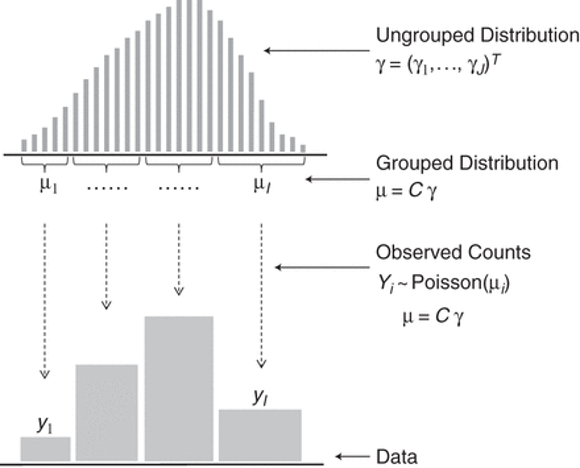
\includegraphics{resources/rizzi-2015-figure_one.png}

}

\caption{Rizzi}

\end{figure}

Rizzi et al., Am J Epidemiol, Volume 182, Issue 2, 15 July 2015, Pages
138--147, https://doi.org/10.1093/aje/kwv020
\end{frame}

\begin{frame}{Methods}
\protect\hypertarget{methods-1}{}
\begin{itemize}
\item
  Models convictions data and population data together to estimate a
  smooth surface of conviction rates
\item
  Means that you probably shouldn't look for disruptions in the time
  series (policy shocks or what have you)
\item
  But you can look at overall trends
\end{itemize}
\end{frame}

\begin{frame}{Modelling Assumptions}
\protect\hypertarget{modelling-assumptions}{}
\begin{itemize}
\item
  This is an unusual (for me at least) use of a statistical model! For
  prediction rather than inference
\item
  Model makes some assumptions:

  \begin{itemize}
  \tightlist
  \item
    ``neighboring elements in \emph{γ} do not differ drastically''
  \item
    ``This smoothness assumption is implemented in a roughness penalty
    on the coefficients \emph{β}''
  \end{itemize}
\item
  There is a penalty term \emph{λ} and what the model does is pick the
  `best' value of \emph{λ} as determined by AIC
\item
  This means that - in the frequentist setting - the final results are
  `optimal' but you might be concerned about propagating uncertainty in
  λ through your analysis (Bayes doesn't have this problem, but has the
  problem of I don't know how to fit this model)
\item
  You can get standard errors for your estimates/confidence intervals
  for the estimated conviction count/rate for each age in each year, but
  these seemed not to make much difference to the results from a quick
  look so I haven't bothered here
\item
  This is because the age categories were coarse at older ages where
  there were also fewer convictions
\end{itemize}
\end{frame}

\begin{frame}{Analysis}
\protect\hypertarget{analysis}{}
\begin{itemize}
\tightlist
\item
  Look at the results visually on the Lexis surface (Minton) and as a
  bunch of line charts
\item
  Calculate relevant summary statistics (mode, median, mean, skew,
  kurtosis)
\item
  I did look into ways of quantifying how different each country's
  age-crime surface was (things like 2D generalizations of
  Kolmogorov-Smirnov tests and that sort of thing), to quantify how
  `similar' the age-crime surfaces are
\item
  Can frame this as either `how similar' (continuous) or `are they
  statistically significantly different from each other' (discrete)
\item
  Problem that the time series are different lengths (for methods like
  Kullback--Leibler divergence at least this is a problem)?
\item
  Methods do exist but seem opaque to me - so I haven't bothered (yet)
\item
  {[}Describe lexis surfaces here and how to read them, describe the
  difference between surfaces approach{]}
\end{itemize}
\end{frame}

\begin{frame}{The lexis surface}
\protect\hypertarget{the-lexis-surface}{}
\begin{figure}

{\centering 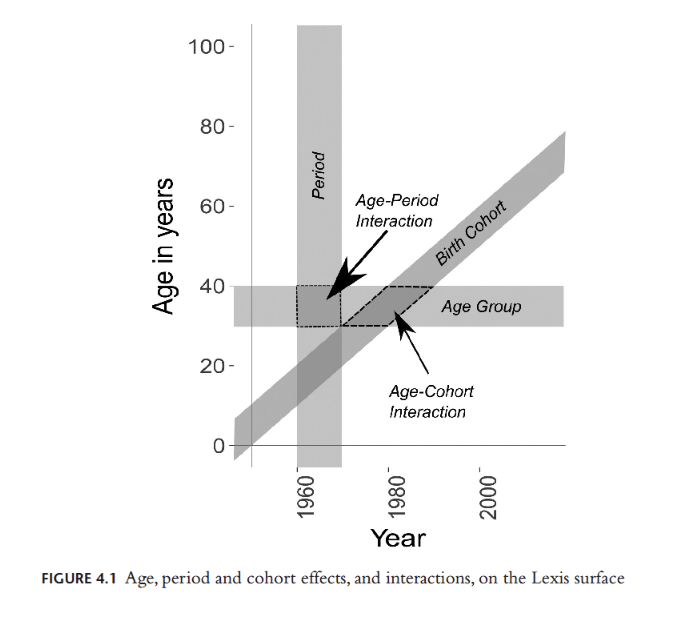
\includegraphics{resources/minton_2020_lexis.png}

}

\caption{Minton}

\end{figure}
\end{frame}

\begin{frame}{Results}
\protect\hypertarget{results}{}
\begin{figure}

{\centering 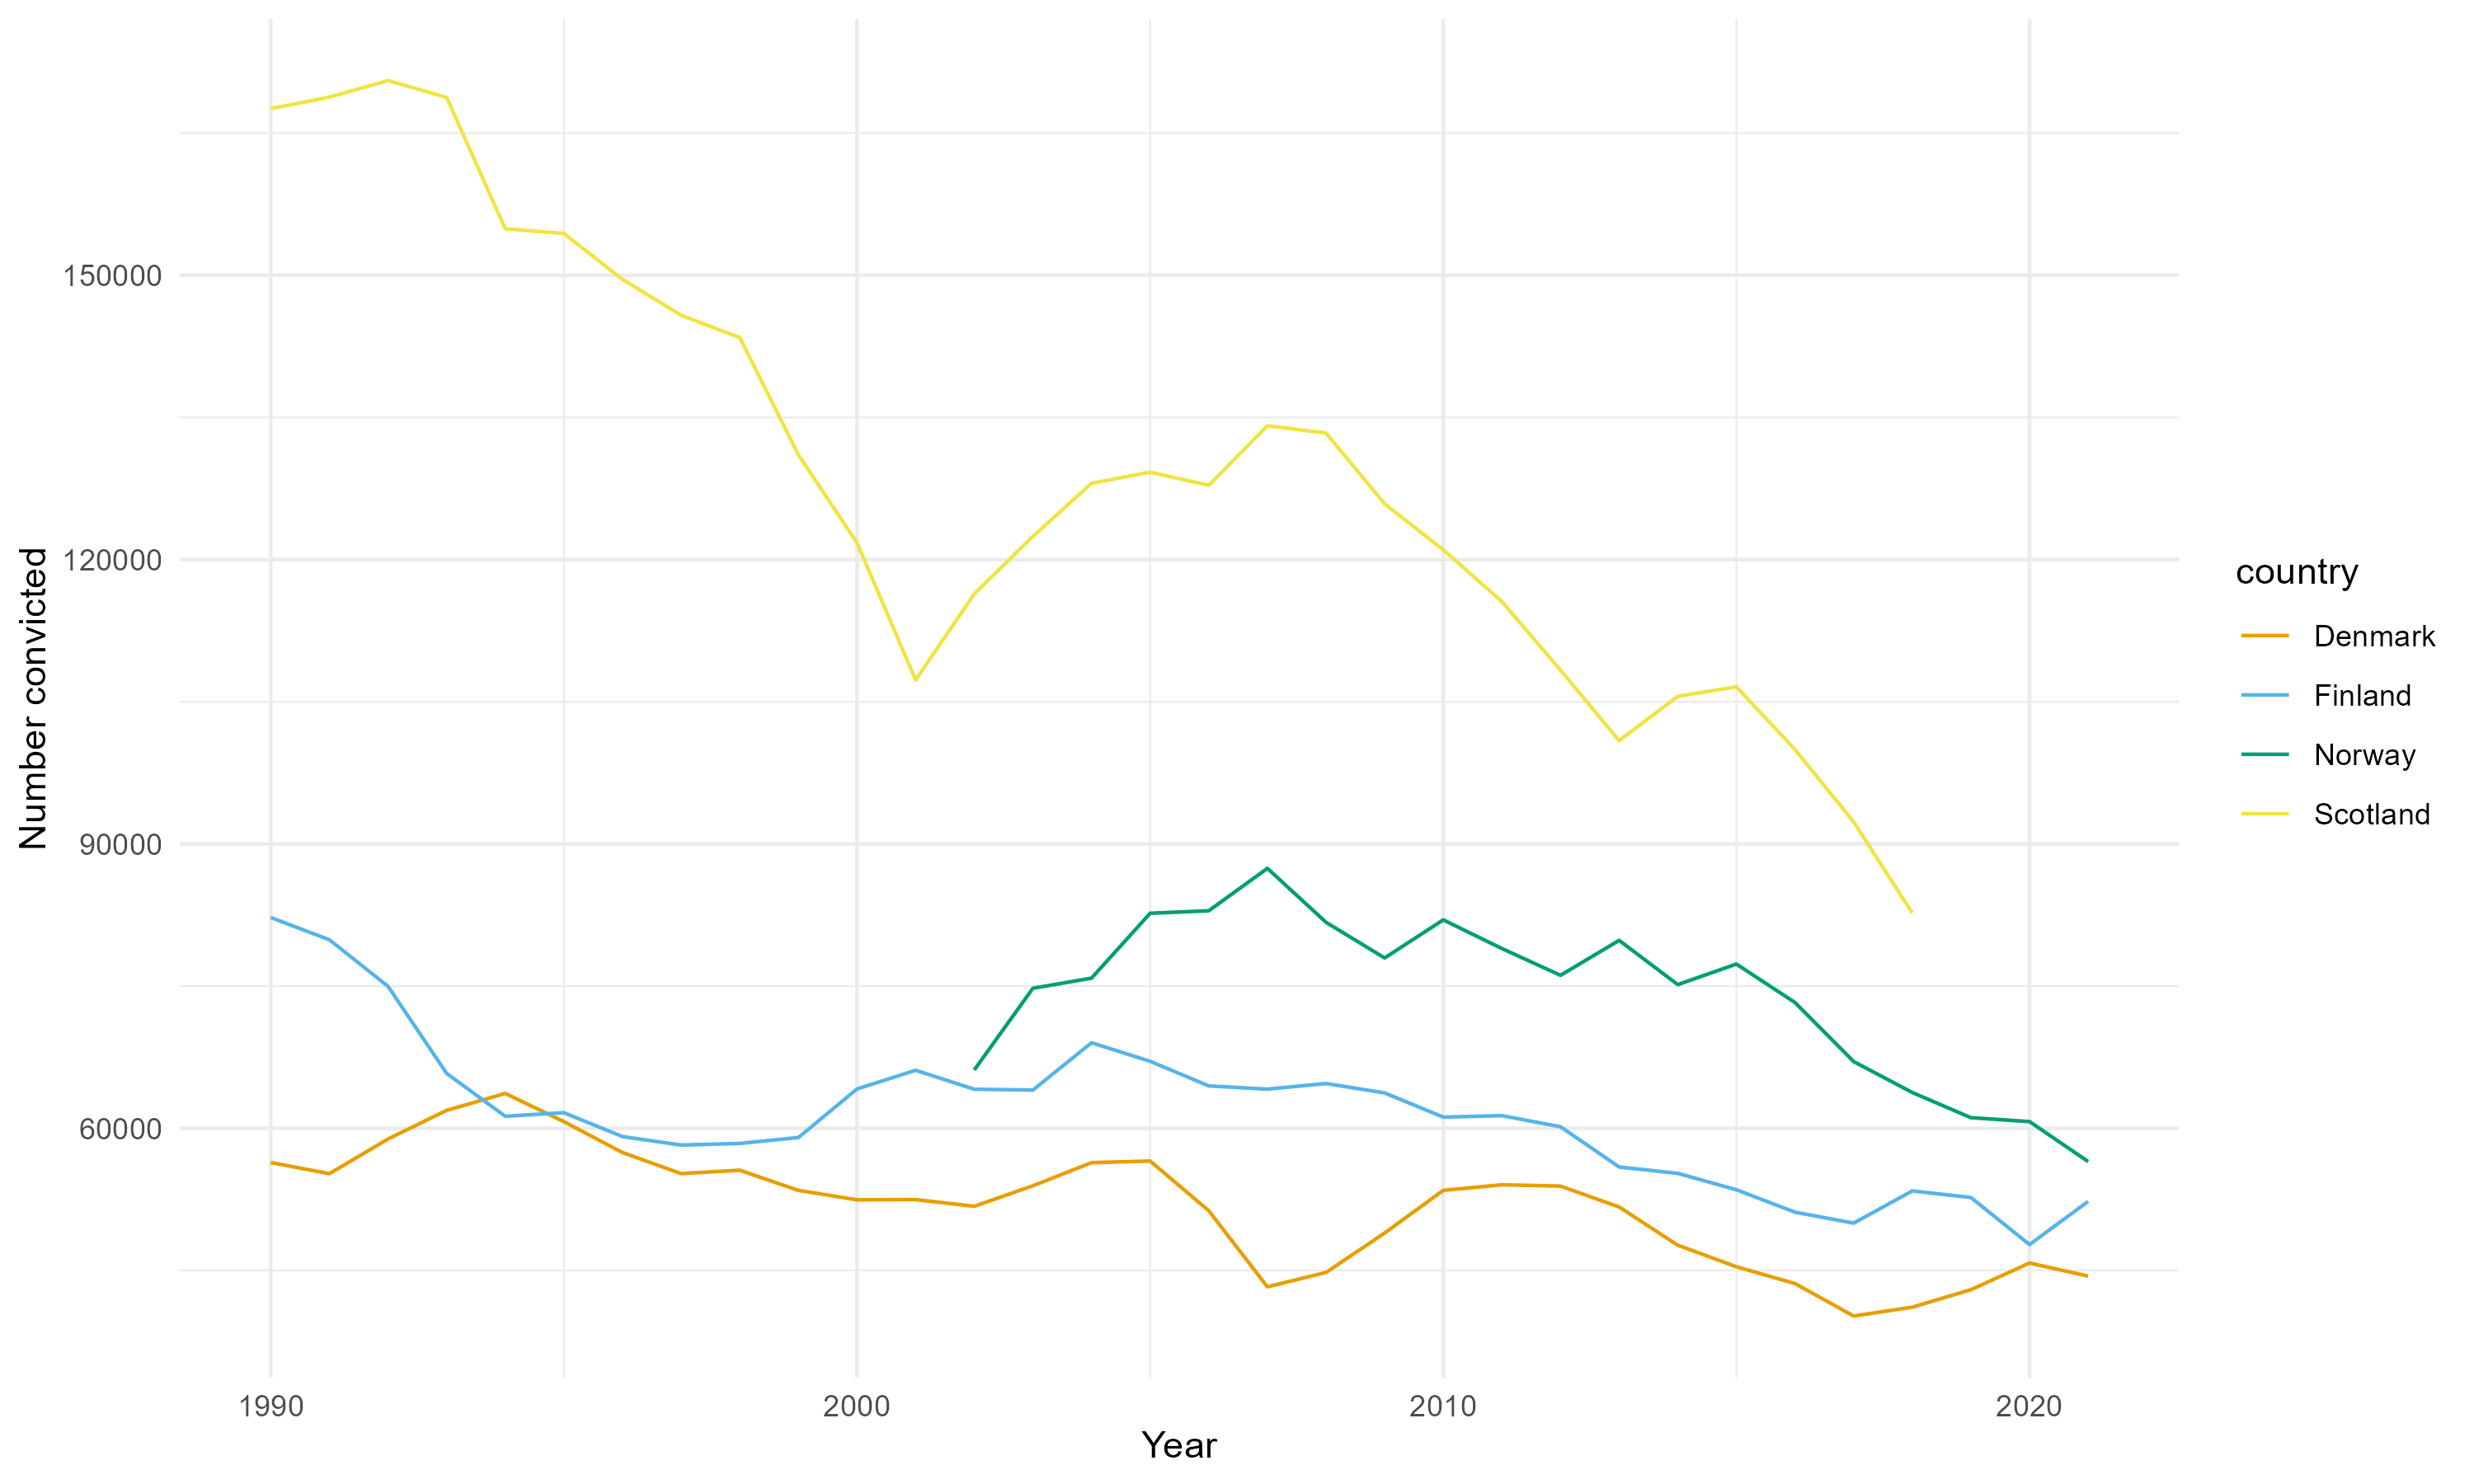
\includegraphics{figures/overall_conviction_trends.png}

}

\caption{trends}

\end{figure}
\end{frame}

\begin{frame}{Comparing countries}
\protect\hypertarget{comparing-countries}{}
\begin{figure}

{\centering \includegraphics{figures/acc_anim.gif}

}

\caption{Anim}

\end{figure}
\end{frame}

\begin{frame}{new page}
\protect\hypertarget{new-page}{}
\begin{figure}

\begin{minipage}[t]{0.50\linewidth}

{\centering 

\raisebox{-\height}{

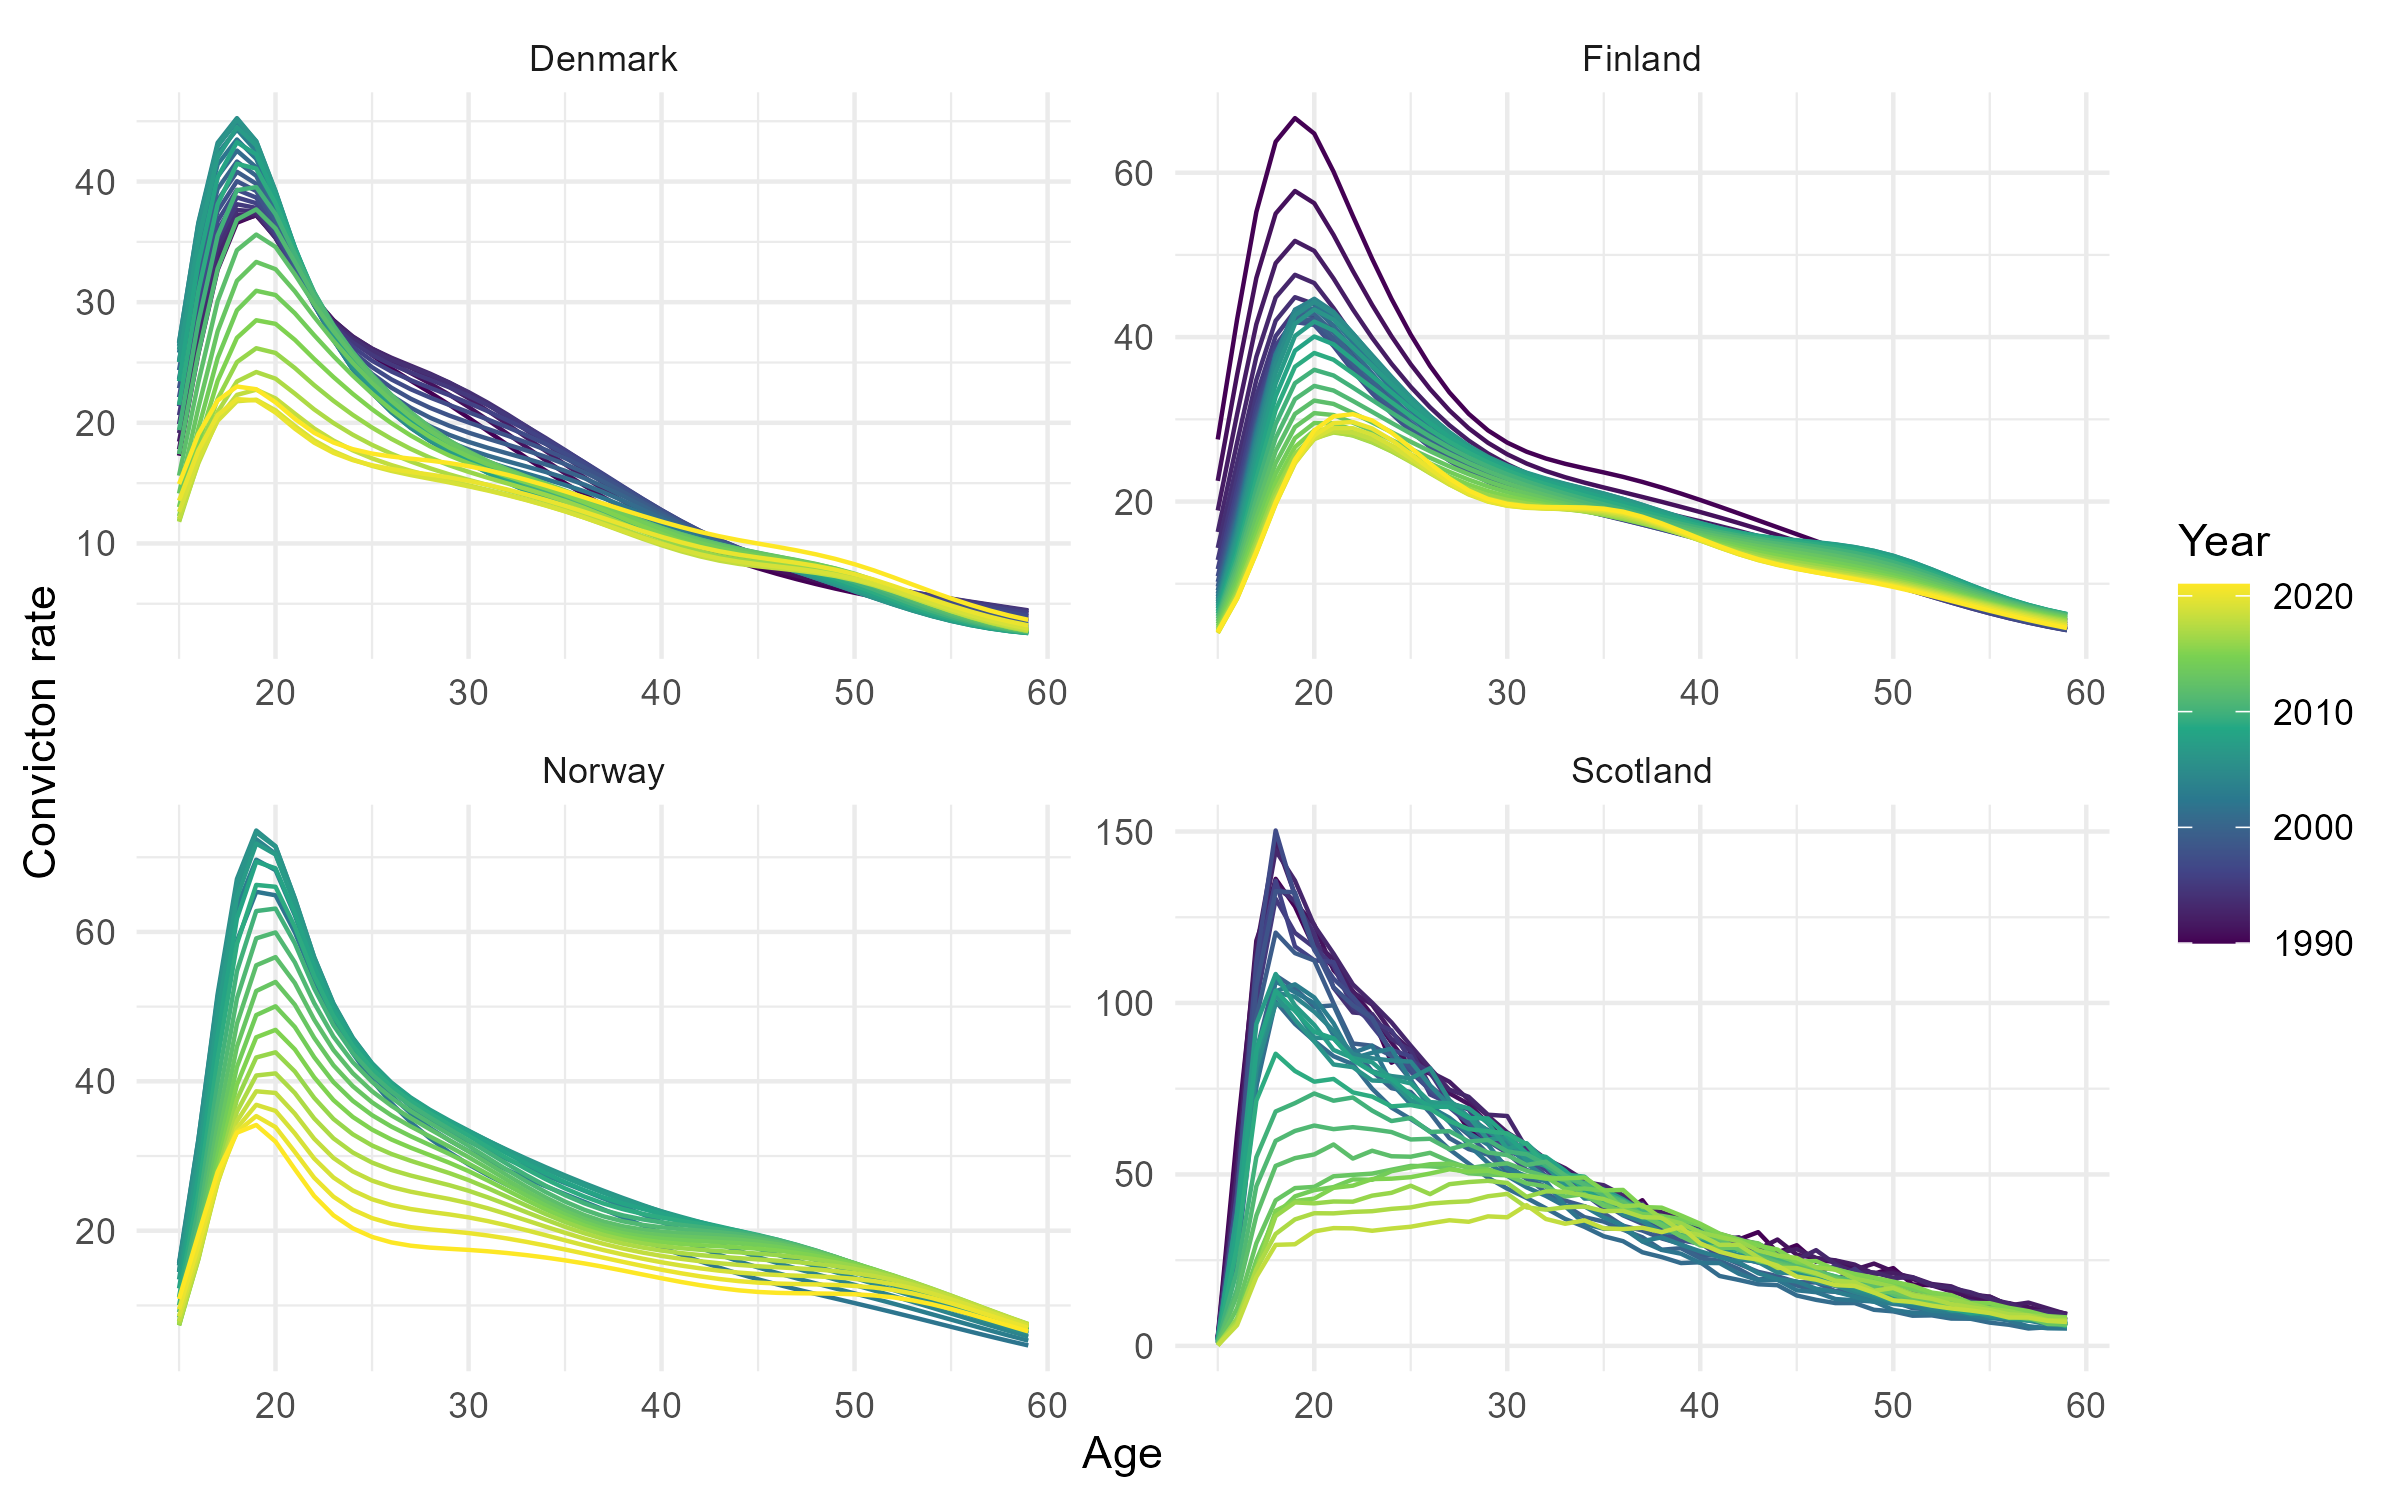
\includegraphics{figures/acc_overall_fig.png}

}

\caption{Age-crime curves}

}

\end{minipage}%
%
\begin{minipage}[t]{0.50\linewidth}

{\centering 

\raisebox{-\height}{

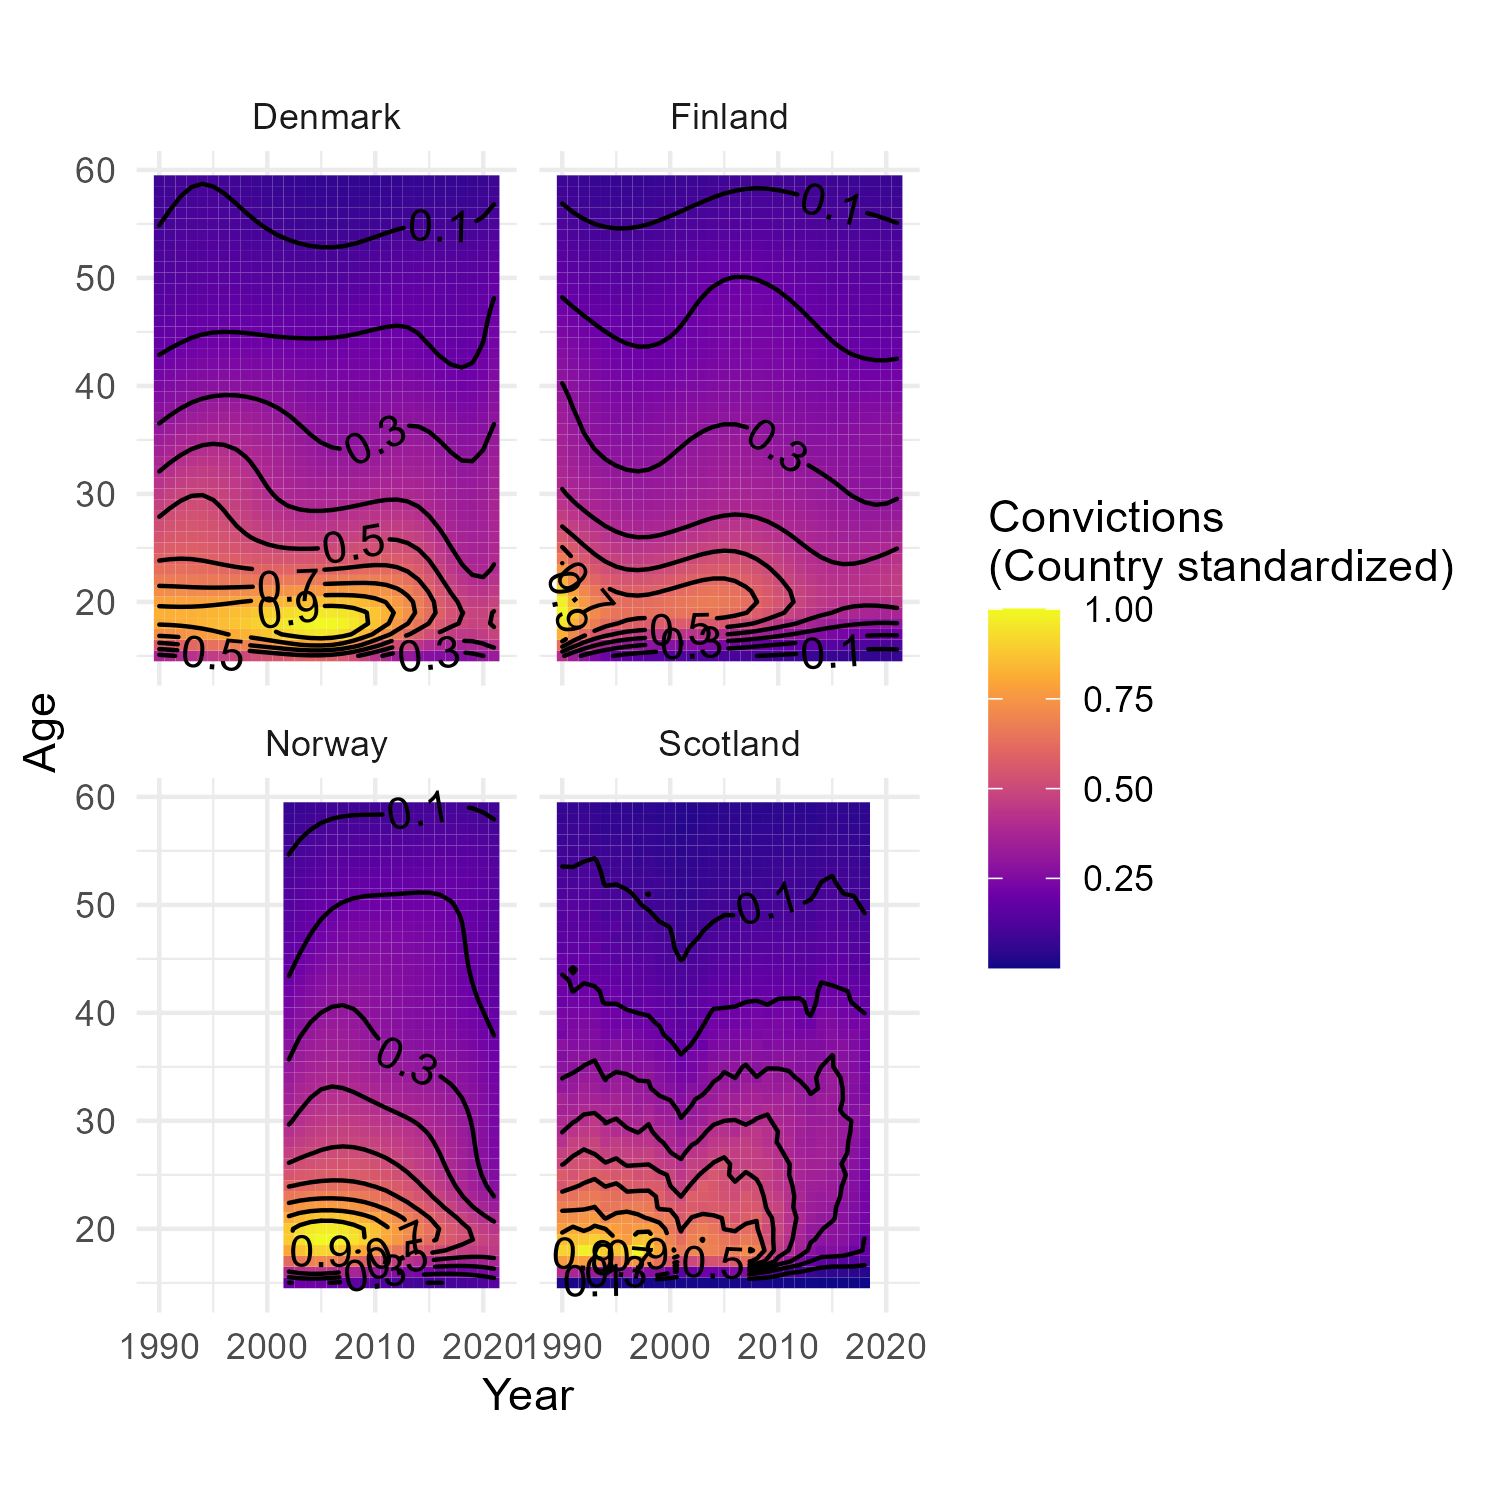
\includegraphics{figures/acc_std_facet.png}

}

\caption{Age-crime curves}

}

\end{minipage}%

\caption{\label{fig-acc}Title}

\end{figure}
\end{frame}

\begin{frame}{ridgeline}
\protect\hypertarget{ridgeline}{}
\begin{figure}

{\centering 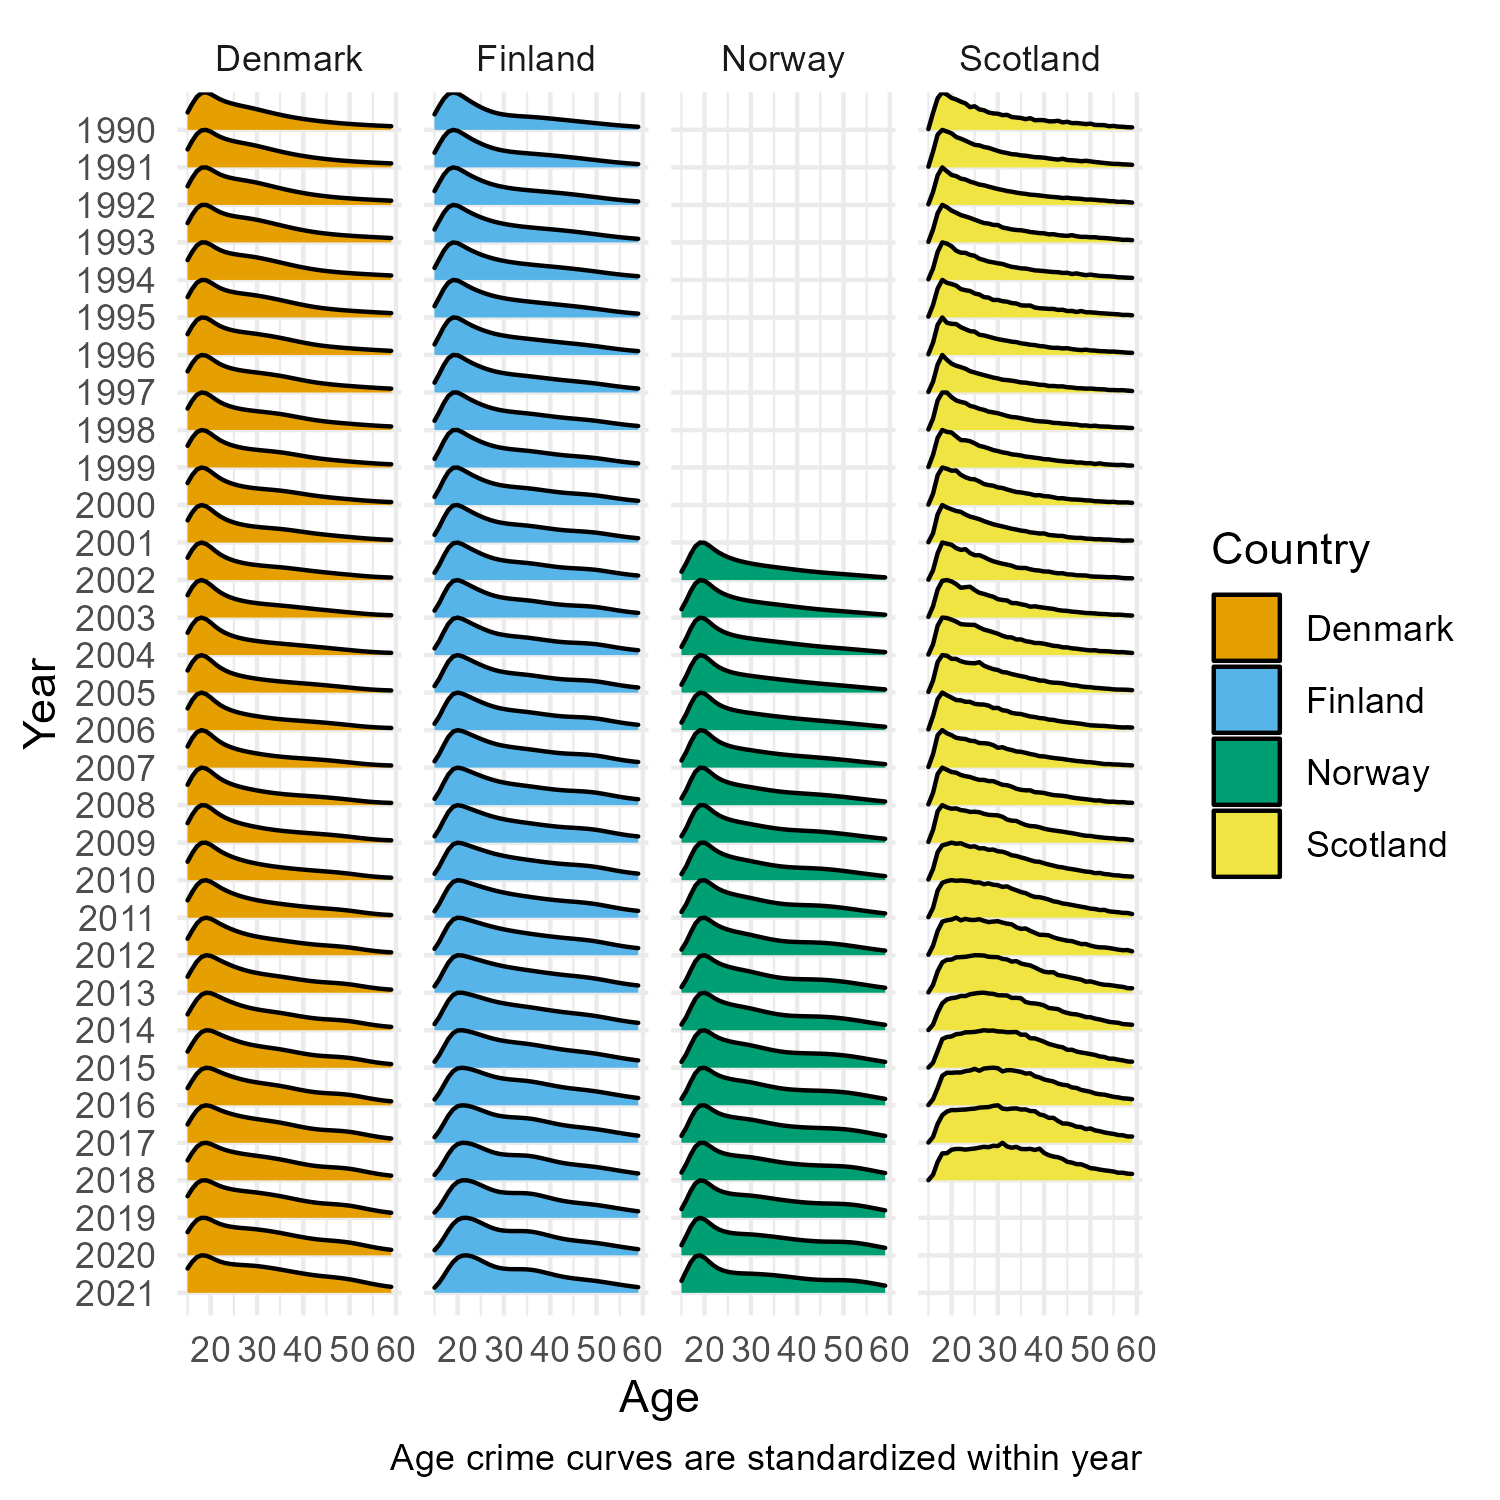
\includegraphics{figures/acc_ridgeline.png}

}

\caption{Age-crime curves ridgelines}

\end{figure}
\end{frame}

\begin{frame}{summary statistics}
\protect\hypertarget{summary-statistics}{}
\begin{figure}

{\centering 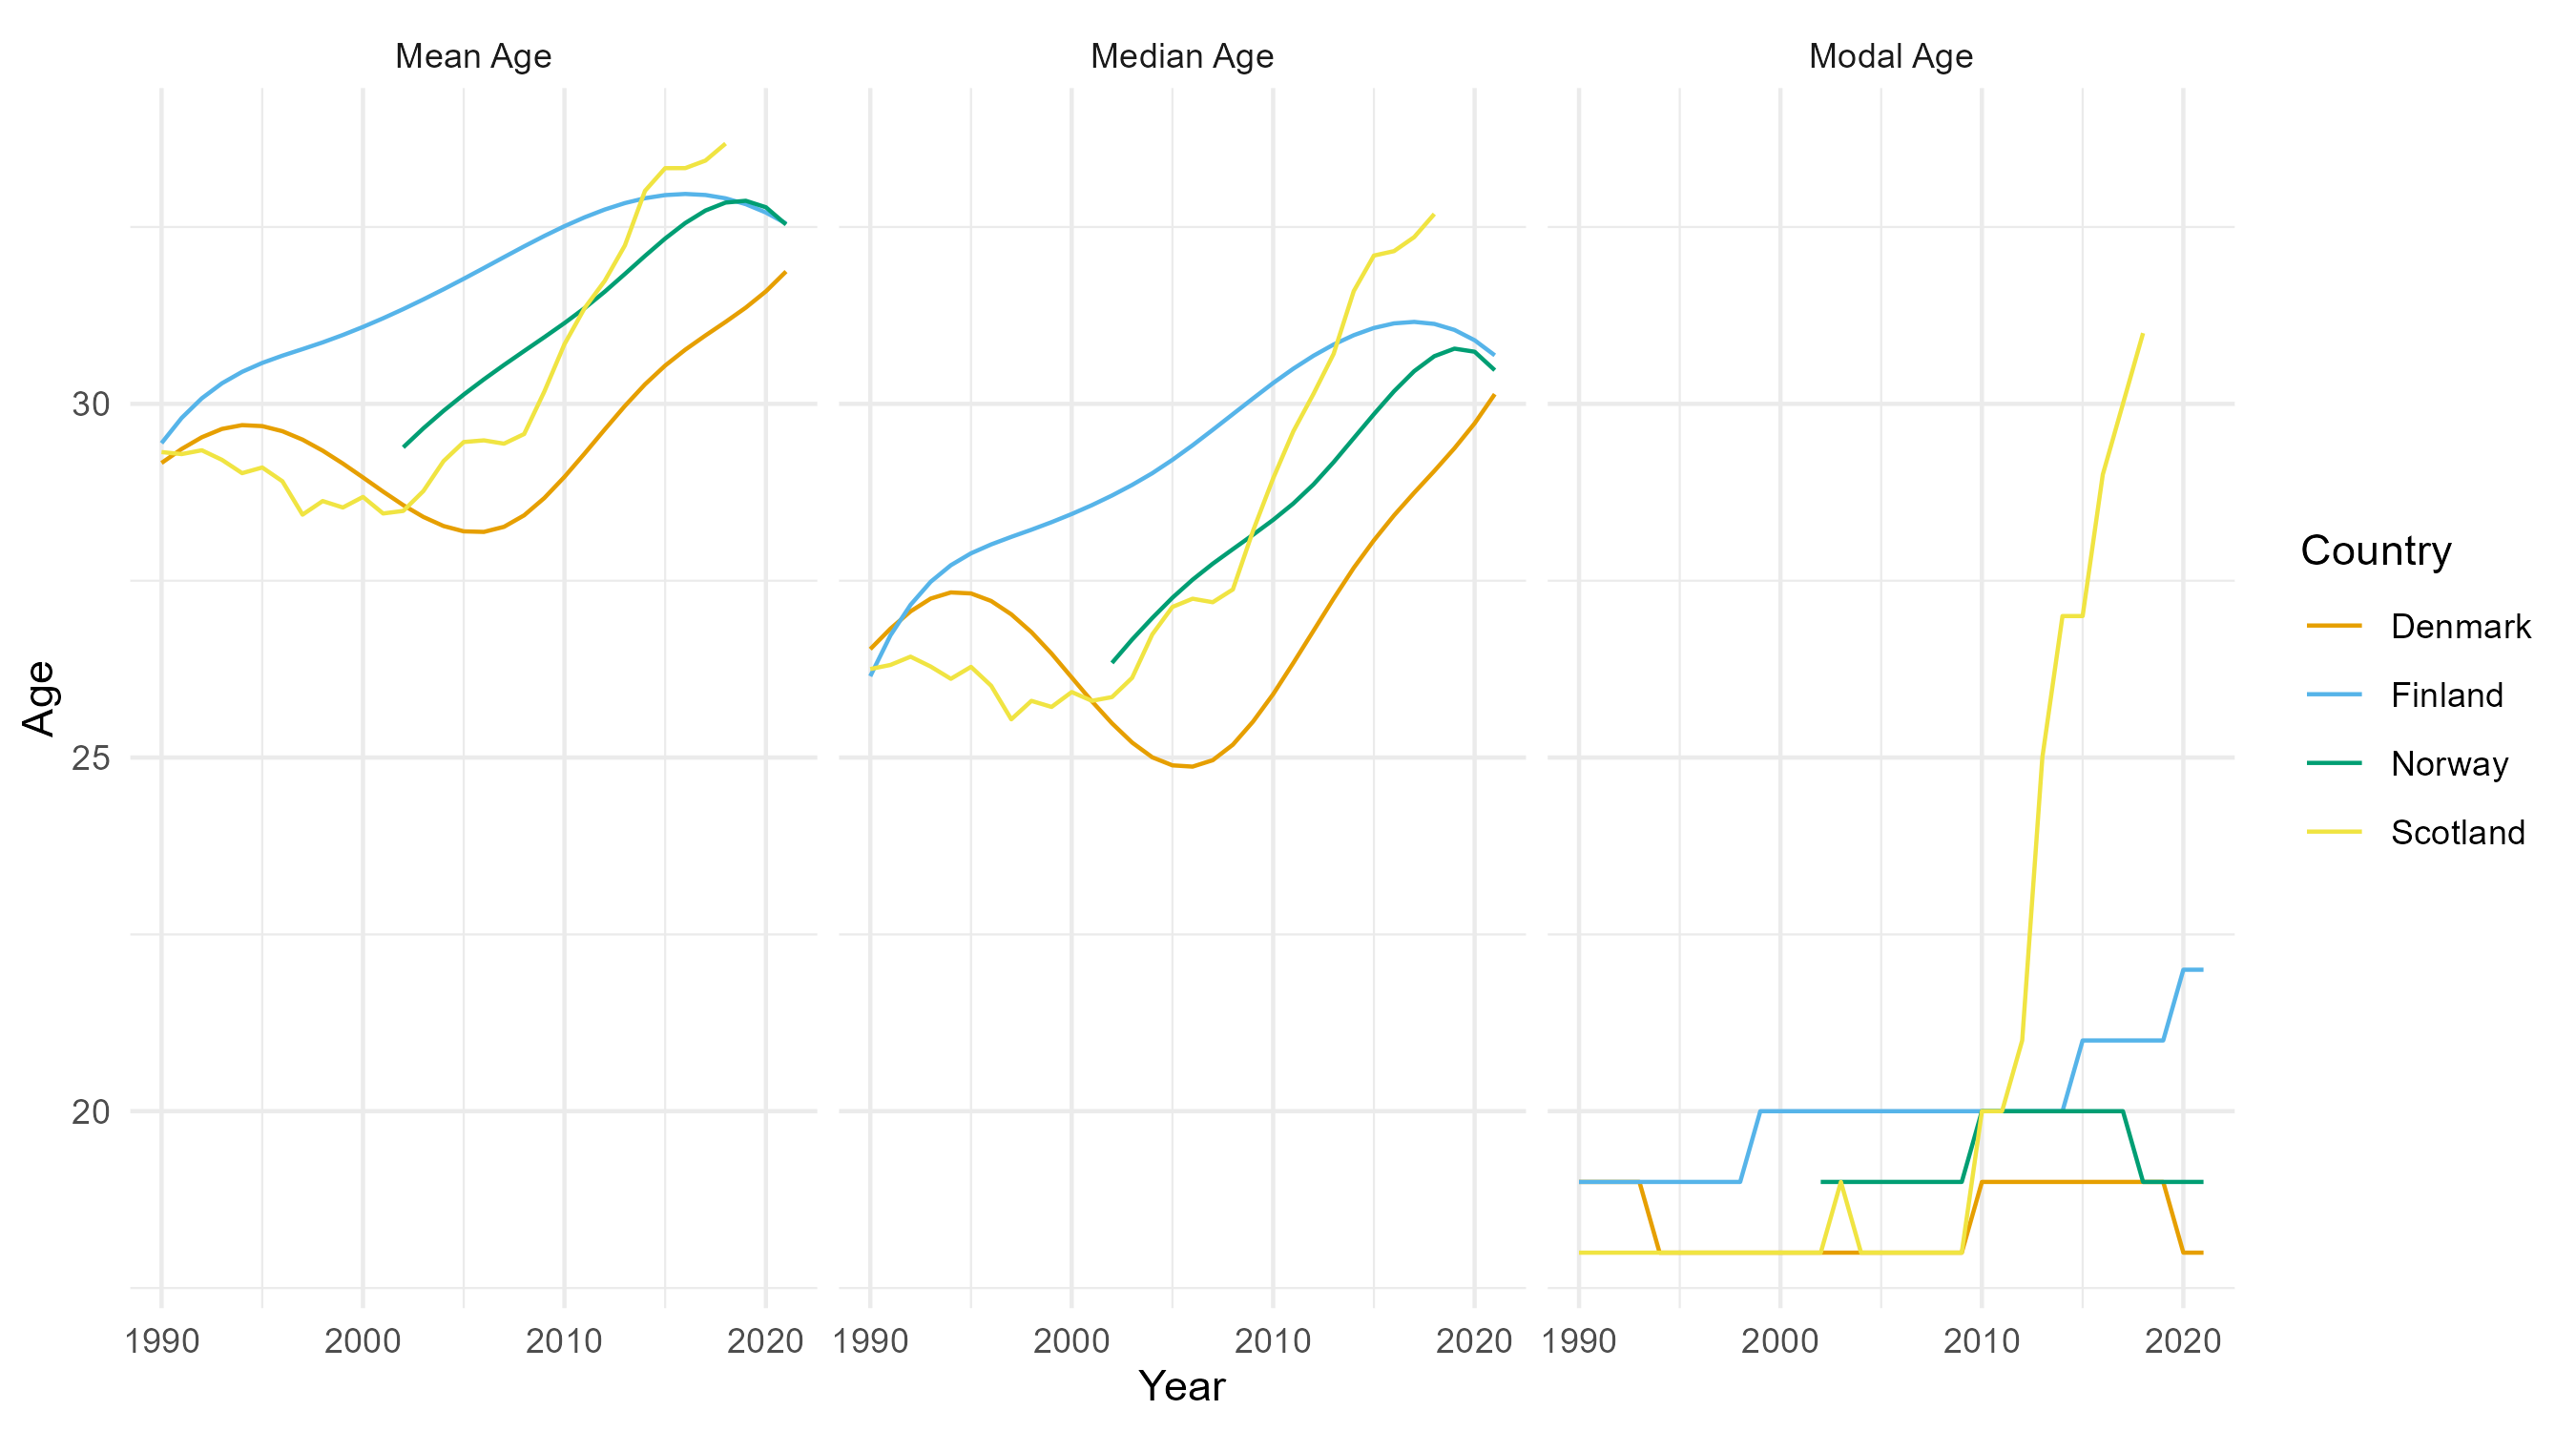
\includegraphics{figures/summary_statistics.png}

}

\caption{Summary statistics}

\end{figure}
\end{frame}

\begin{frame}{age index}
\protect\hypertarget{age-index}{}
\begin{figure}

\begin{minipage}[t]{0.50\linewidth}

{\centering 

\raisebox{-\height}{

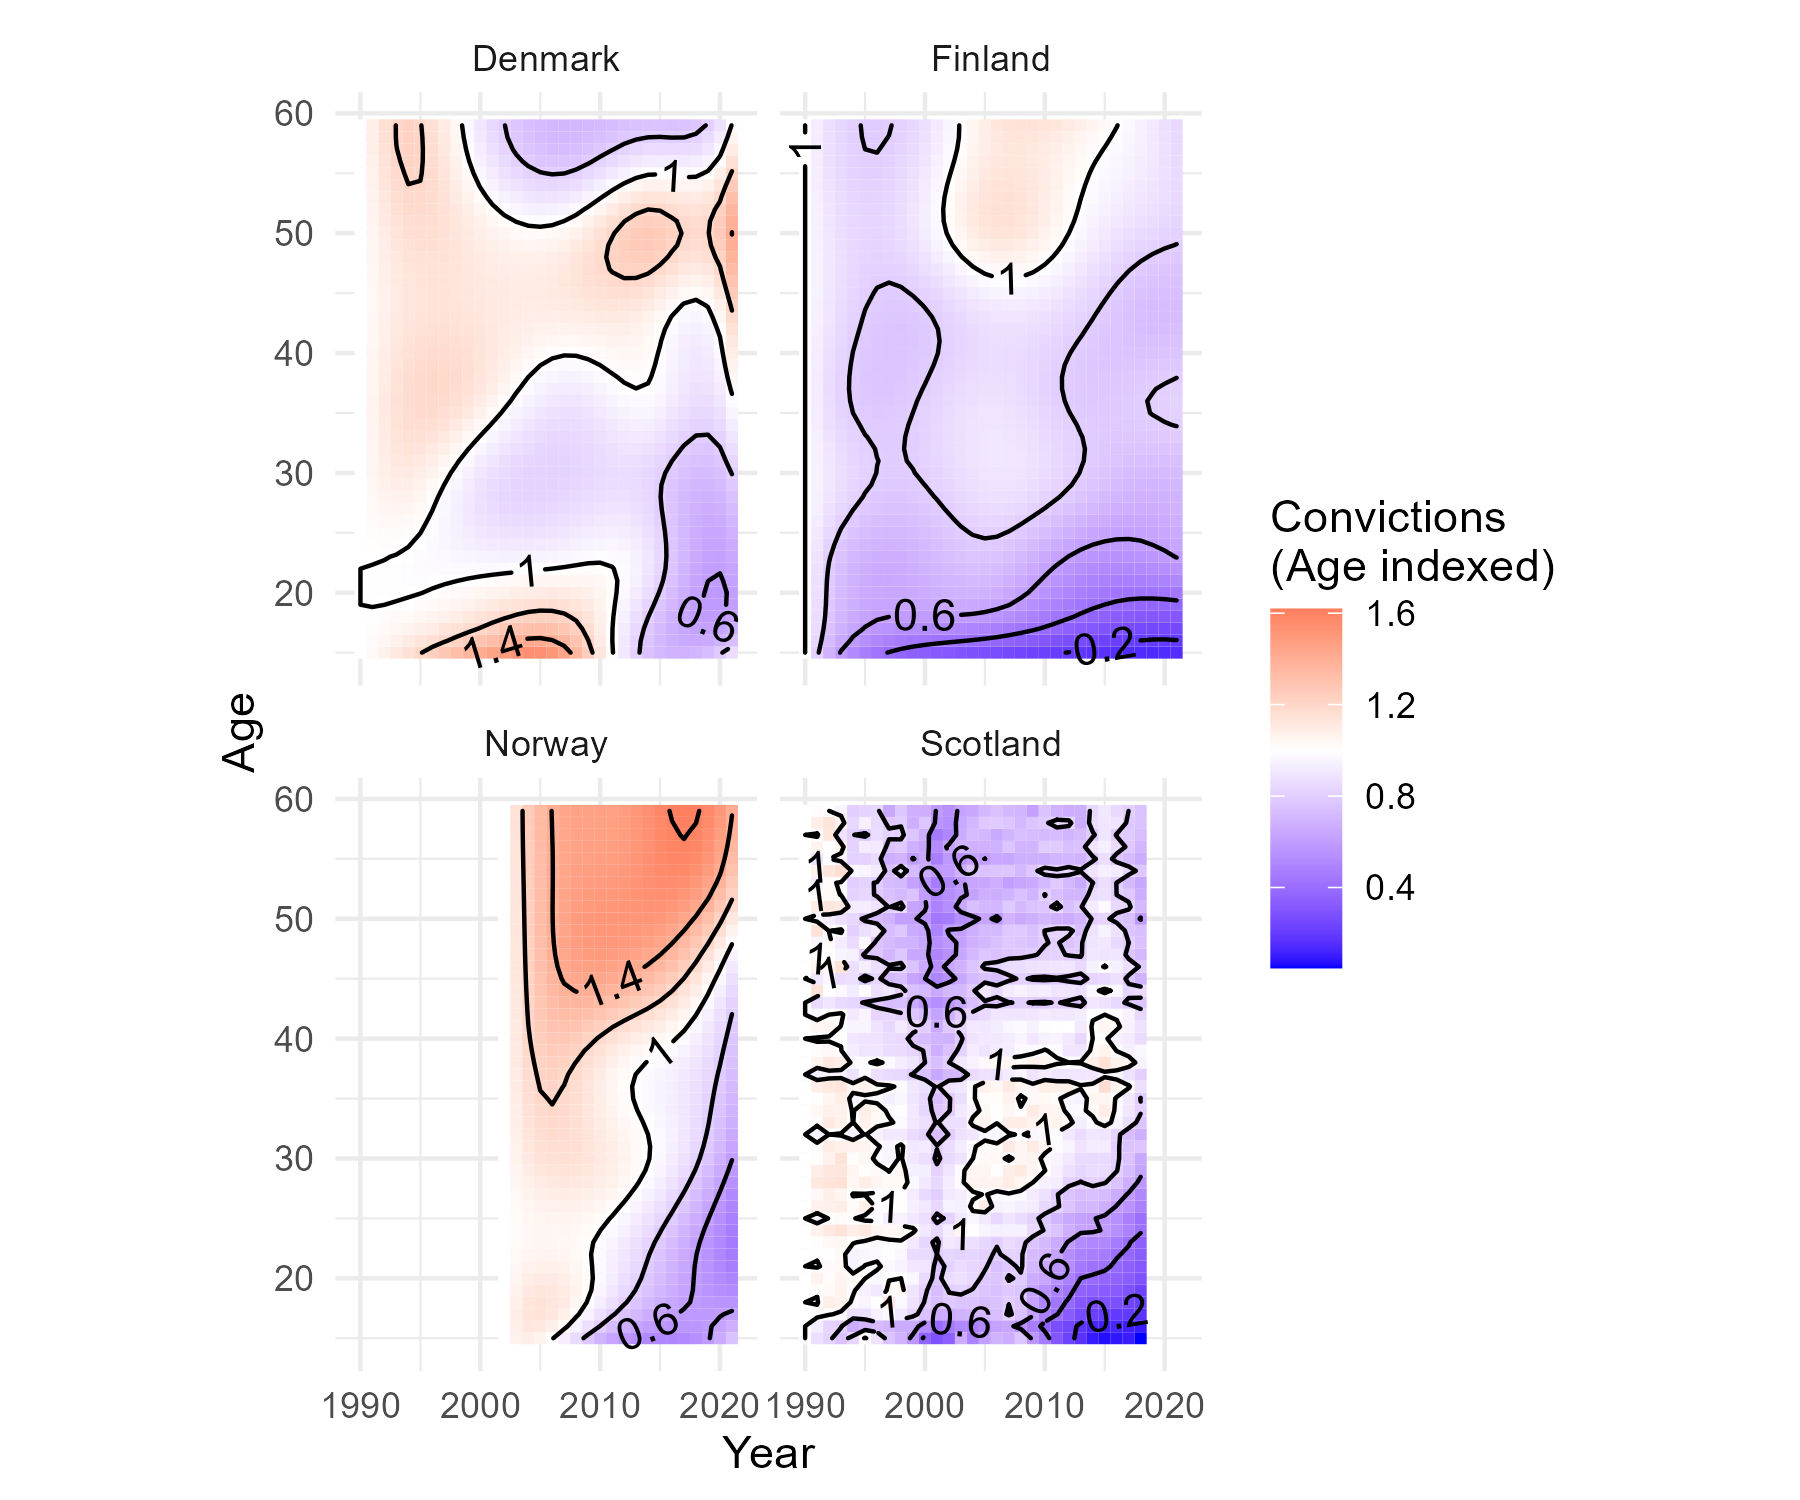
\includegraphics{figures/acc_age_index_surface.png}

}

}

\subcaption{\label{fig-surus}Acc age index lexis}
\end{minipage}%
%
\begin{minipage}[t]{0.50\linewidth}

{\centering 

\raisebox{-\height}{

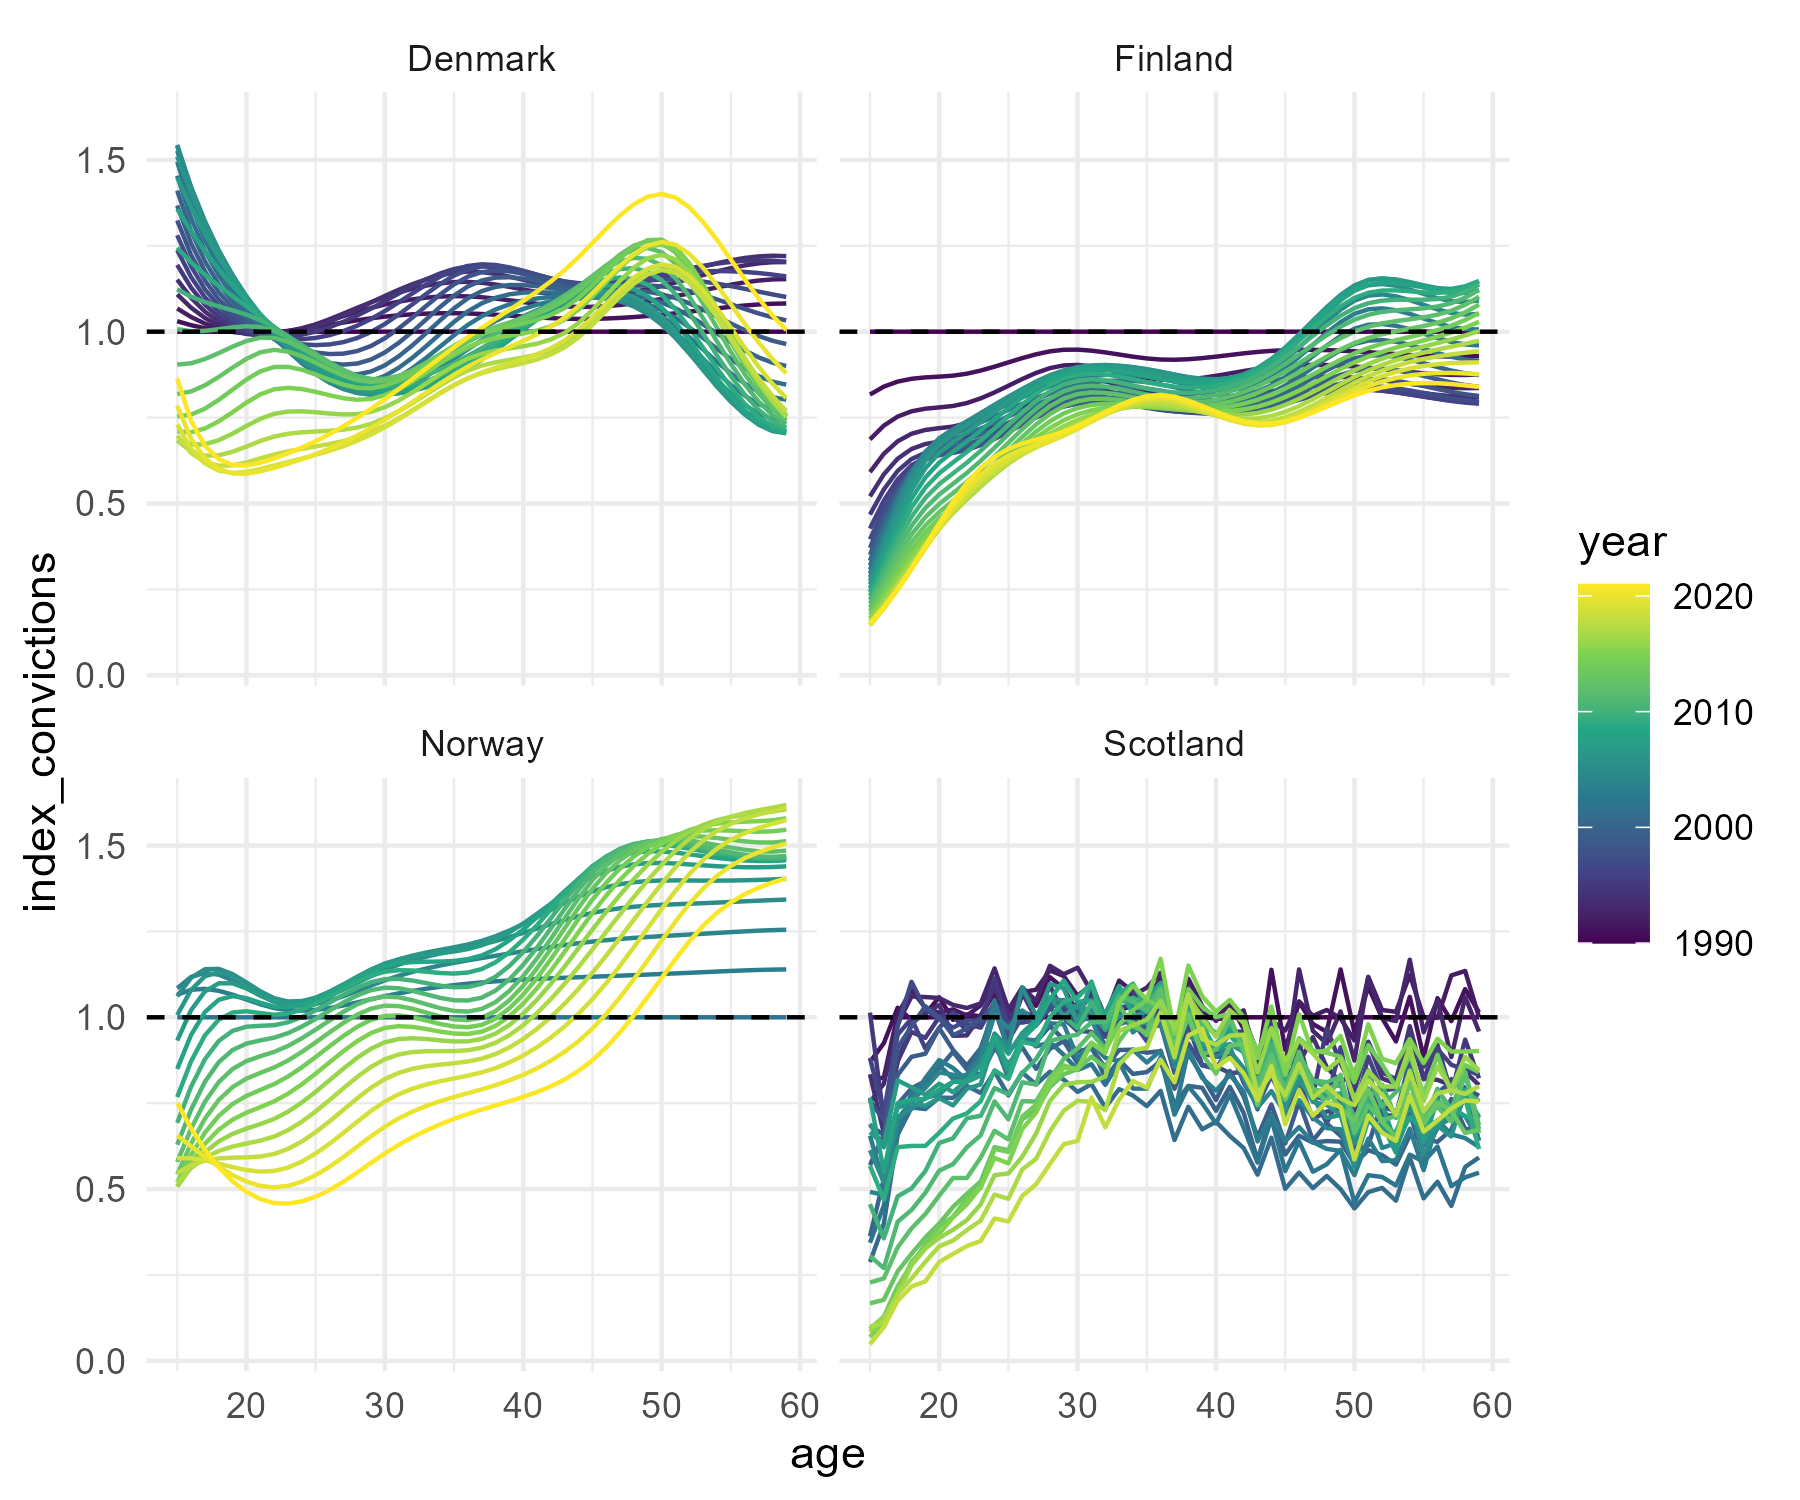
\includegraphics{figures/acc_age_index_facet.png}

}

}

\subcaption{\label{fig-hanno}Acc age index facet}
\end{minipage}%

\caption{\label{fig-acc-index}Some plots}

\end{figure}
\end{frame}

\begin{frame}{Conclusions}
\protect\hypertarget{conclusions}{}
\begin{itemize}
\tightlist
\item
  The crime drop \emph{is} (mostly?) a youth crime drop
\item
  Timings of biggest falls in youth convictions (cohorts born around
  1990ish) are pretty consistent?
\item
  Don't see the same fall in for people at older ages
\item
  But only really see the increases in convictions 30s-40s in Scotland
\item
  So maybe you're happy if you're the `generation sensible' people
\item
  Scotland does seem like an odd fit with these comparators
\end{itemize}
\end{frame}

\begin{frame}{Conclusions}
\protect\hypertarget{conclusions-1}{}
\begin{itemize}
\tightlist
\item
  If you believe in the invariance these about the age-crime curve, you
  almost lose by winning - I'd say that three of the four countries
  showed pretty `classic' age-crime curves throughout the period
  analysed, but one didn't
\item
  This is implies that there are between country differences in how the
  age-crime curve has changed over time
\item
  But the whole point of the invariance thesis is that it's invariance
  across time and place - so the fact that the change in the age-crime
  curve in Scotland seems very different than in Denmark, Finland and
  Norway is (I would argue) a \emph{bad} thing for the invariance thesis
\item
  This initial analysis raises lots of questions about\ldots{} crime
  types, other demographics (gender, ethnicity, income\ldots{} etc) that
  could be answered by more bespoke data
\item
  Having done this analysis for (some of) Northern Europe, I think maybe
  an even more maximalist approach would be better - and can extend this
  comparison to anywhere that publishes data on age and conviction
\end{itemize}
\end{frame}



\end{document}
